\begin{exercises} 
  \item  Consider the differential equation
    $$
    \frac{dy}{dt} = t-y.
    $$
    
    \ba
    	\item Sketch a slope field on the plot below:
    \begin{center}
      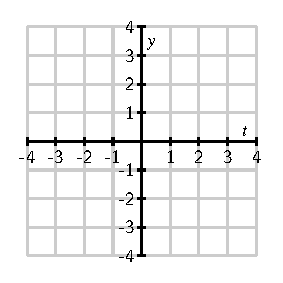
\includegraphics{figures/7_2_ex_1.eps}
    \end{center}

    \item  Sketch the solutions whose initial values are $y(0)= -4, -3, \ldots, 4$.  

    \item  What do your sketches suggest is the solution whose initial
    value is $y(0) = -1$?  Verify that this is indeed the solution to
    this initial value problem.

    \item  By considering the differential equation and the graphs you
    have sketched, what is the relationship between $t$ and $y$ at a
    point where a solution has a local minimum?
    \ea
  
  \item Consider the situation from problem 2 of Section~\ref{S:7.1.DEIntro}:  Suppose
    that the population of a particular species is  
    described by the function $P(t)$, where $P$ is expressed in
    millions.  Suppose further that the population's rate of change is
    governed by the differential equation 
    $$\frac{dP}{dt} = f(P)
    $$
    where $f(P)$ is the function graphed below.

    \begin{center}
      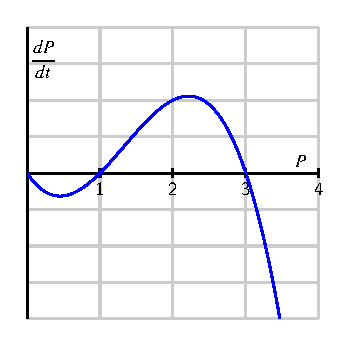
\includegraphics{figures/7_1_threshold.eps}
    \end{center}

    \ba
    \item  Sketch a slope field for this differential equation.  You do
    not have enough information to determine the actual slopes, but
    you should have enough information to determine where slopes are positive, negative, zero, large, or small, and hence determine the qualitative
    behavior of solutions.

    \item Sketch some solutions to this differential equation when the
    initial population $P(0)>0$.

    \item  Identify any equilibrium solutions to the differential equation and classify them as stable
    or unstable.

    \item  If $P(0)>1$, what is the eventual fate of the species?

    \item  if $P(0)<1$, what is the eventual fate of the species?

    \item  Remember that we referred to this model for population growth
    as ``growth with a threshold.''  Explain why this characterization makes sense by considering
    solutions whose inital value is close to 1.  
	\ea
	
  \item The population of a species of fish in a lake is $P(t)$ where
    $P$ is measured in thousands of fish and $t$ is measured in
    months.  The growth of the population is described by the
    differential equation
    $$
    \frac{dP}{dt} = f(P) = P(6-P).
    $$

   \ba
   \item  Sketch a graph of $f(P) = P(6-P)$ and use it to determine the
    equilibrium solutions and whether they are stable or unstable.
    Write a complete sentence that describes the long-term behavior of
    the fish population.

    \item Suppose now that the owners of the lake allow fishers to
    remove 1000 fish from the lake every month (remember that $P(t)$
    is measured in {\em thousands} of fish).  Modify the differential
    equation to take this into account.  Sketch the new graph of
    $dP/dt$ versus $P$.  Determine the new equilibrium solutions and
    decide whether they are stable or unstable.  

    \item  Given the situation in part (b), give a description of
    the long-term behavior of the fish population.

    \item  Suppose that fishermen remove $h$ thousand fish per month.  
    How is the differential equation modified?  

    \item  What is the largest
    number of fish that can be removed per month without eliminating the fish
    population?  If fish are removed at this maximum rate, what is the
    eventual population of fish?
    
    \ea

  \item Let $y(t)$ be the number of thousands of mice that live on a
    farm;  assume time $t$ is measured in years.\footnote{This problem is based on an ecological analysis
    presented in a research paper by C.S. Hollings:  The Components of
    Predation as Revealed by a Study of Small Mammal Predation of the
    European Pine Sawfly, {\em Canadian Entomology} {\bf 91}: 283-320.  }

    \ba
    \item  The population of the mice grows at a yearly rate that is twenty times 
    the number of mice.  Express this as a differential equation.

    \item At some point, the farmer brings $C$ cats to the farm.  The
    number of mice that the cats can eat in a year is
    $$M(y) = C\frac{y}{2+y}$$
    thousand mice per year.  Explain how this modifies the
    differential equation that you found in part a).

    \item
     Sketch a graph of the function $M(y)$ for a single cat $C=1$ and
    explain its features by looking, for instance, at the behavior of
    $M(y)$ when $y$ is small and when $y$ is large.

    \item Suppose that $C=1$.  Find the equilibrium solutions and
    determine whether they are stable or unstable.  Use this to
    explain the long-term behavior of the mice population depending on
    the initial population of the mice.

   \item Suppose that $C=20$.  Find the equilibrium solutions and
    determine whether they are stable or unstable.  Use this to
    explain the long-term behavior of the mice population depending on
    the initial population of the mice.

    \item  What is the largest number of cats for which the mice
    population can survive?

\ea


    
        
\end{exercises}
\afterexercises
